% !TeX root=../main.tex
\chapter{موقعیت‌یابی و کالیبراسیون به صورت همزمان یک ربات کابلی با در نظر گرفتن کابل‌ها به صورت جسم صلب}

\section{مقدمه}
همانطور که در فصل قبل ذکر شد، اگرچه سنسورهای فضای مفصل سریع و ارزان هستند، اما زمانی که از آنها برای اندازه‌گیری مقادیر مجری نهایی استفاده می‌شود، دقت مدل  سینماتیکی برای تعیین دقت قابل دستیابی بسیار مهم است. 
علاوه بر این، در زمینه همجوشی و ترکیب اندازه‌گیری‌ها، هم‌ثبت کردن داده ها \cite{hall1997introduction} اولین گام اساسی است. به عبارت دیگر، حسگرها باید اندازه‌گیری‌های خود را در یک مختصات یکپارچه ارائه دهند. اهمیت هم‌ثبت به دلیل فرض اساسی نویز گاوسی با میانگین صفر در الگوریتم‌های ترکیب داده‌ها می باشد. 
نکته قابل توجه دیگر برای ربات های آسان نصب، لزوم بی نیازی الگوریتم کالیبراسیون پیشنهادی به حسگرهای گران  قیمت و یا حسگرهایی که نیاز به تعمیر و نگهداری سطح بالایی هستند می باشد. علاوه بر این، فرآیند کالیبراسیون باید به اندازه‌ای ساده باشد که اجرای آن در مکان‌های مختلف آسان و سریع باشد.  
با اینکه کالیبراسیون موضوعی است که بسیاری از پژوهشگران به آن علاقه‌مند هستند، اما مفهوم بهره‌گیری از چندین حسگر برای بهبود نتایج کمتر مورد توجه قرار گرفته است. علاوه بر این، الگوریتم کالیبراسیون یکپارچه و قابل گسترش در ادبیات برای ربات‌های کابلی وجود ندارد. 

از طرفی دیگر، افزون بر مفهوم و ضرورت کالیبراسیون در این ربات ها، موقیت یابی این ربات ها نیز مورد توجه بسیاری قرار گرفته است. 
همانطور که پیش تر بیان شد، الگوریتم های بسیاری در راستای ترکیب حسگرها و همچنین کاهش زمان پردازش برای موقعیت یابی ربات به صورت زمان-واقعی در انواع دیگر ربات ها همچون ربات های خودران مورد استفاده قرار گرفته است. 

آنچه در ادامه این رساله مورد توجه قرار می گیرد، آدرس دهی جامع برای حل تمامی موارد بیان شده در بالا می باشد. بدین منظور، رویکردی معرفی می شود که در وهله اول مسائل کالیبراسیون و موقعیت یابی را به صورت یک مسئله یکپارچه در یک قاب ببیند و سپس انعطاف پذیری الگوریتم مجال افزودن حسگرهای اضافی را فراهم نماید. چنین رویکردی نه تنها انجام دو فرآیند مجزای کالیبراسیون و موقعیت یابی را به یک فرآیند ترکیب شده و همزمان تبدیل می کند، بلکه به راحتی می تواند به دیگر الگوریتم های ادبیات موضوع افزوده شود. نتیجه این رویکرد علاوه بر افزایش دقت نهایی این فرآیندها، مفهومی حقیقی تر به آسان نصب بودن به این دسته از ربات های کابلی می بخشد. الگوریتم پیشنهادی برای فرمول بندی این مسئله با آدرس دهی آنچه مورد نیاز ما است، الگوریتم گراف عامل می باشد. ویژگی های منحصر به فرد این الگوریتم در حل مسائل تنک مانند مسئله موقعیت یابی و نقشه برداری به صورت بر خط باعث استفاده زیادی از این فرمول بندی برای طیف وسعی از کاربرد های رباتیکی در سال های اخیر شده است.

در این فصل حل مسئله موقیت یابی و کالیبراسیون به صورت هزمان برای یک ربات کابلی فروتحریک با در نظر گرفتن فرض اساسی صلب بودن کابل ها مورد بررسی قرار می گیرد. در حالی که فرمول بندی مسئله با در نظر گرفتن این فرض بسیار ساده تر می شود، تا زمانی که شکم دهی کابل ها ناشی از جرم آنها بسیار ناچیز باشد، قابل قبول خواهد بود. حل این مسئله برای کابل شکم دار منجر به ایجاد چالش هایی می گردد که در فصل آتی به صورت مفصل به آنها پرداخته می شود و در نهایت با رویکرد پیشنهادی بار دیگر حل می گردد. 

\section{روش های مرسوم موقعیت یابی و کالیبراسیون}
به صورت کلی،انتظار می رود چنانچه به یک ربات در دنیای واقع یک ورودی مشخص اعمال شود، با اعمال همان ورودی به مدل پاسخی یکسان دریافت شود. با این حال همواره وجود نامعینی ها و عدم دقیق بودن پارامتر های مدل در واقعیت ما را از رسیدن به چنین پاسخی ایده آل باز می دارد. این نامعینی ها می تواند ناشی از تقریب هایی باشد که در مدل داریم و یا پدیده هایی که در مدل سازی مورد توجه کامل قرار نگرفته اند. جنس این نامعینی ها می تواند ریشه در سینماتیک ربات و یا دینامیک آن باشد. فرآیند کالیبراسیون می تواند این نامعینی ها را در جهتی کاهش دهد که پاسخ هایی که از مدل و ربات در پیاده سازی واقعی دریافت می کنیم، کاهش پیدا کند. آنچه در این کار مورد بررسی قرار گرفته است کالیبراسیون سینماتیکی می باشد. شکل فلان نمایش بلوکی از یک فرآیند کالیبراسیون سینماتیکی بنا بر تعریف بیان شده می باشد. همانطور که در این شکل مشاهده می شود آنچه به عنوان خطا در نظر گرفته می شود تفاوت خروجی هایی می باشد که ناشی از مدل سینماتیکی ربات (در اینجا سیتماتیک مستقیم) و ربات واقعی در فضای کاری ربات، با یک ورودی مشترک در فضای مفصلی آن می باشد. 

\begin{figure}
	\centering
	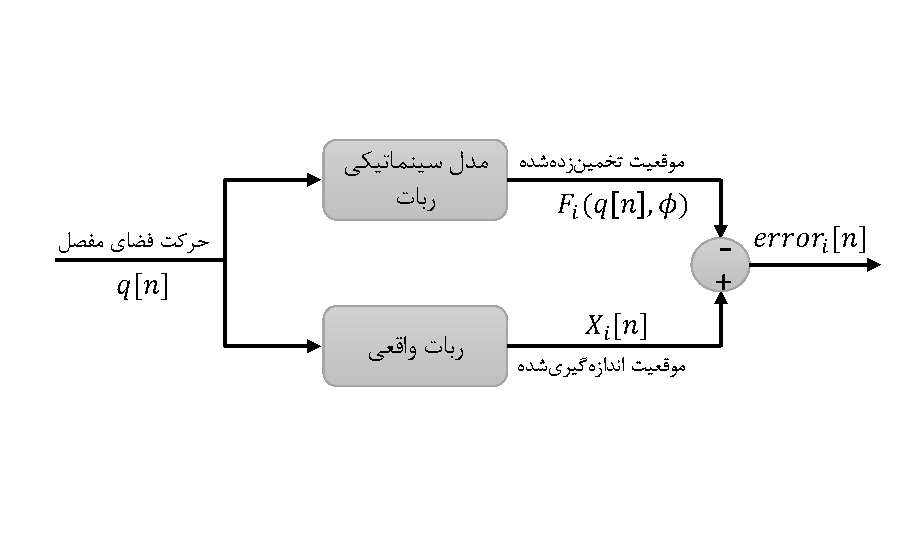
\includegraphics[width=0.8\linewidth, trim={0cm 2.2cm 0cm 2.2cm}, clip]{img/kinematic_model_error}
	\caption{}
	\label{fig:kinematicmodelerror}
\end{figure}


با نگاهی به آخرین تحقیقات بر روی مسيله کالیبراسیون ربات ها، ایجاد یک مسئله بهینه سازی و حل آن برای یافتن مقادیر دقیق این پارامتر های سینماتیکی و دینامیکی ربات مرسوم می باشد
\cite{elatta2004overview,ida2019automatic,ida2022identification,ida2021dynamics}.

 
 
 
 
 
 
 
 
 
 
 
 
 
 
 
 
 
 
 
 
 
 
 
 
 
 
 
 
 